\chapter{Coarse-grained Cross Modal Retrieval}
\label{cha:scan}
In Chapter \ref{cha:relatedworks}, we discussed several models proposed to solve the image-text alignment task. However, they all have drawbacks in terms of different aspects. In this chapter we explain the \textbf{S}tacked \textbf{C}ross \textbf{A}ttentio\textbf{n} Model (SCAN) \cite{scan} and applied it on performing coarse-grained cross-modal retrieval task. 
%% SHURONG: we didn't compare this method with others on our datasets, no?[corrected]
Followed by discussing how it excel the image-text alignment task and why we choose to investigate it to solve the problem later in the task of coarse-grained cross modal retrieval for artworks.

The structure of this chapter is as follows. Section 3.1 gives an introduction and motivation of SCAN. Section 3.2 explains the structure and methodologies used in SCAN, also how all its components iterates with each other. Section 3.3 briefly discusses the strengths of the adopted model for coarse-grained cross-modal retrieval. Section 3.4 illustrates the preliminary experimental results on our artwork datasets and the achievement of SCAN. Section 3.5 summarises this chapter.


%% [done]Shurong: remove the motivation part or a brief sentence saying that SCAN is prove very effective in image-text alignment. 
%%[solved]In this part, it's better the images from the original paper can be replaced by your own. (Move the evaluation metrics in chapter 4 introduction to this chapter.) 
%%Give some insights into the bad examples about why the model does not work for them
\section{Introduction}

There are several models proposed recently to solve the task of cross modal retrieval, and many have achieved excellent accomplishments. Lee, et al. \cite{scan} uses the proposed \textbf{S}tacked \textbf{C}ross \textbf{A}ttentio\textbf{n} (SCAN) to find all potential alignments between the image area and the words, thereby calculating the similarity between the graphics and the text. Existing methods perform fixed-step attention inference so that only a limited semantic alignment can be found at a time, and SCAN can find all possible semantic alignments at the same time. Since the number of semantic alignments varies among different images and sentences, the corresponding relationship inferred by the Stacked Cross Attention method is more comprehensive, thereby making the image-text matching more interpretable.

Also, this method used some of the currently available optimisation methods, such as the use of hard-negative, triplet ranking loss, etc. SCAN is proved to be very effective in image-text alignment task, thus, in this chapter, we employ SCAN on our coarse-grained cross modal retrieval task.

%% ShURONG:This can be the motivation why you use this model and can be put in the beginning? It's not proper to put it here because we actually didn't really compare it with other methods on our own dataset, thus this advantage is only attested on natural images and also a reason why we use this model [done]

We explain the structure of SCAN model in the next sections.

\section{Image Feature Extraction}
Before we perform any cross modal retrieval and alignment between image and text, we need to firstly extract features from images. There are many models we have discussed before in Section \ref{cha:relatedworks}, here we use one of the most widely used model called faster R-CNN to both extract the top-$k$ image regions from an image and represent the image regions of interest as a continuous vector as in the work done by Anderson, et al. \cite{bottomup}. It proposes a top-down and bottom-up attention model method, which is applied to the related issues of visual scene understanding and prominent question answering system.  

The article mentions the use of faster R-CNN to employ a bottom-up attention model - that we adopted. Different from the traditional faster R-CNN, \cite{bottomup} uses not only the object detector but also the attribute classifier for each region of interest, so that a binary description of the object (attribute, object) can be obtained. This description is more suitable for practical applications. Bottom-up attention model also allows the overlap of interest frames through the preset threshold, which can understand the image content more effectively.


%% SHURONG: give an overall introduction like this? for example, we use faster-rcnn introduced in chapter 2 to both extract the top-k image regions from an image and represent the image regions as a continous vector as in \cite{bottom up}. and then introduce how bottom up use faster-rcnn differently with the classical one (it adds instance attributes in visual genome if I remember correctly, double check this:)) [done]

%% SHURONG; This paragraph seems not related?[deleted]
%Although this work \cite{bottomup} does not mention the Encoder-Decoder framework, which is the most widely used in the current research, the task of the bottom-up attention model is to obtain the image interest area. Extracting image features is similar to feature encoding the image to achieve the encoding stage Task; and the top-down attention model is used to learn to adjust the feature weights, realise the ``timely attention'' of image content, and generate descriptions word by word, equivalent to the decoding stage.

\subsection{Why Adopt Faster R-CNN?}

\begin{figure}[h!]
\centering
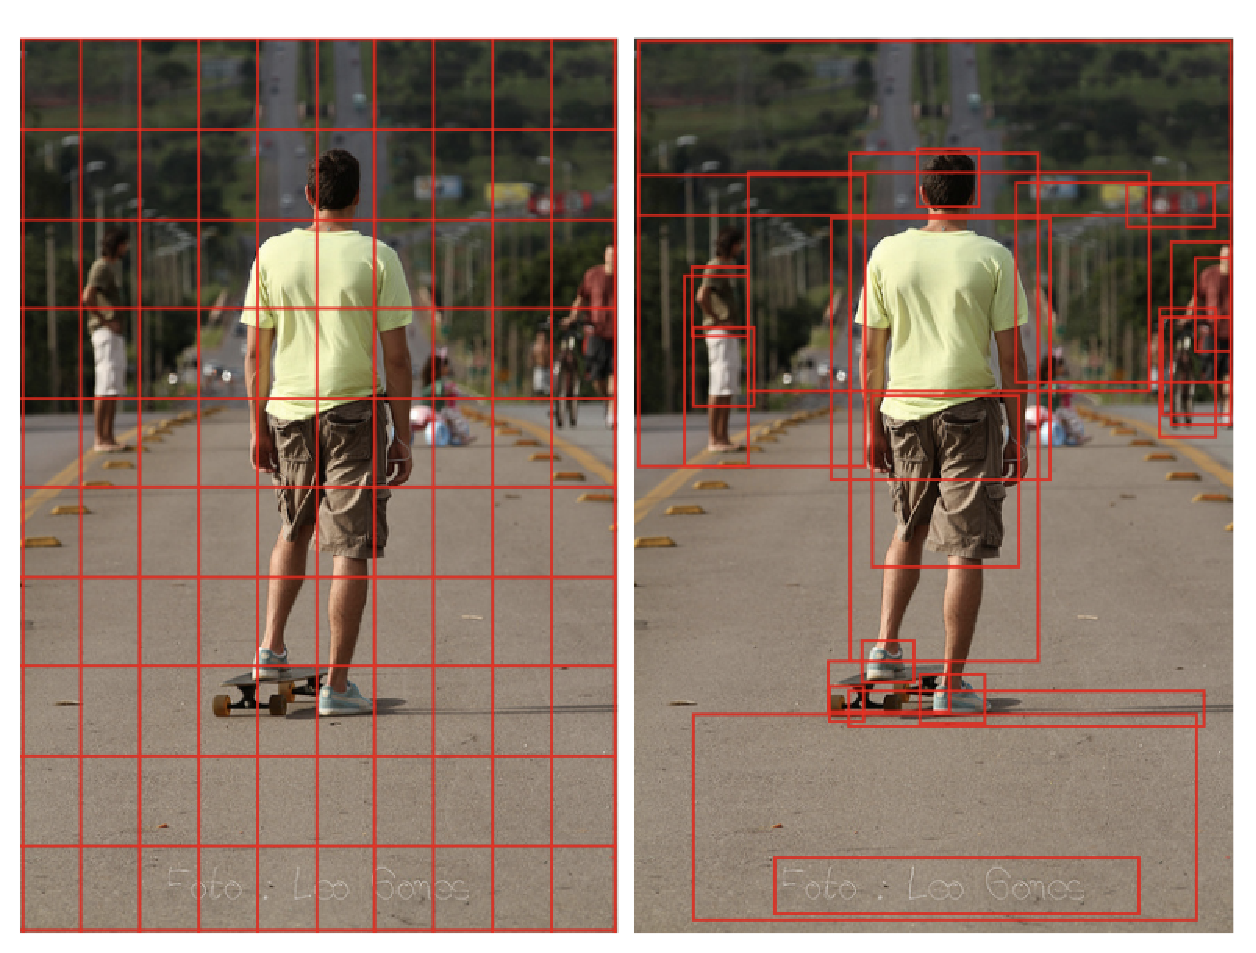
\includegraphics[width=.5\textwidth]{whyfasterrcnn.pdf}
\caption{Faster R-CNN with attention comparing to CNN \cite{bottomup}}
\label{fig:fasterrcnnbottomup}
\end{figure}

It can be seen from the Figure \ref{fig:fasterrcnnbottomup} that using CNN demands more features than R-CNN, and many features are often worthless. The object detection method of R-CNN first captures the interest region for an image, then applies an object detector to each interest region, so that the image category can be accurately obtained; the CNN method expects the input of an entire image and is used for broad sample classification, which are often complicated and computationally intensive. Besides, faster R-CNN improves on previous generations of R-CNN methods and earns the ability to recognise almost all objects with only one input, which significantly improves the processing efficiency.

\subsection{Bottom-Up Attention Model}

From Figure \ref{fig:bottomup} below, it can be seen that the difference from the prior works is that the set of thresholds allows overlapping of interest frames, which can more effectively understand the image content. In this model, not only the object detector but also the attribute classifier is used for each region of interest, so that a binary description of the object \verb|(attribute, object)| can be obtained. This description is proved more suitable for real-world applications.

\begin{figure}[h!]
\centering
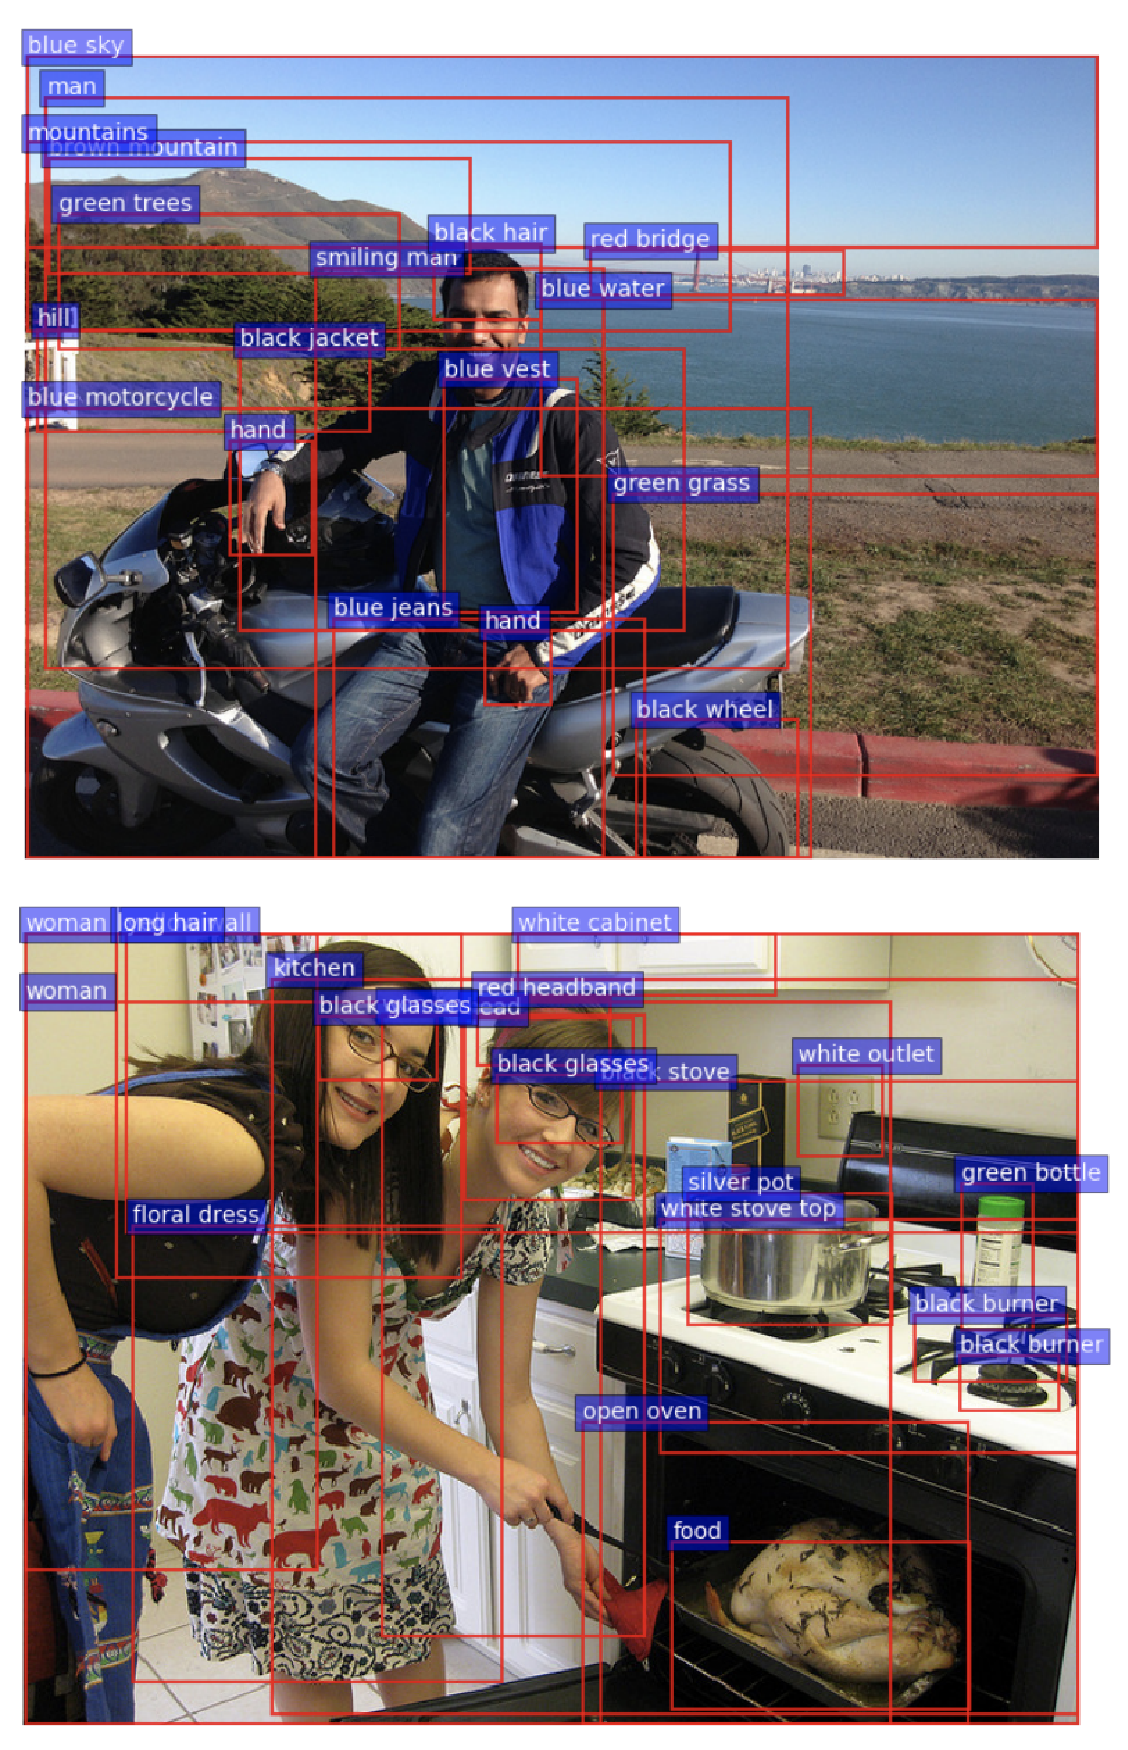
\includegraphics[width=.5\textwidth]{bottomup.pdf}
\caption{What bottom-up attention model captures? \cite{bottomup}}
\label{fig:bottomup}
\end{figure}

\section{SCAN Model}
In this section, we discuss SCAN model with a brief introduction on its structure, followed by in-depth explanations on each specific stages - what is happening behind and why?

\subsection{Brief Structure}
\begin{enumerate}
    \item Use bottom-up attention mechanism \cite{bottomup} to detect the image area and extract the features of the image area;
    \item Map the words in the sentence and their sentence context to feature vectors;
    \item Stacked Cross Attention is used to deduce the similarity of images and text by aligning image regions and word features;
    \item The loss function of SCAN focuses on the hardest negative image-text pairs in each batch (that is, the most unmatched image-text pairs).
\end{enumerate}

Next, we are going to explain each stage in detail.

\subsection{Image-Text Matching}

The process is shown below in Figure \ref{fig:scan1}.

\begin{figure}[h!]
\centering
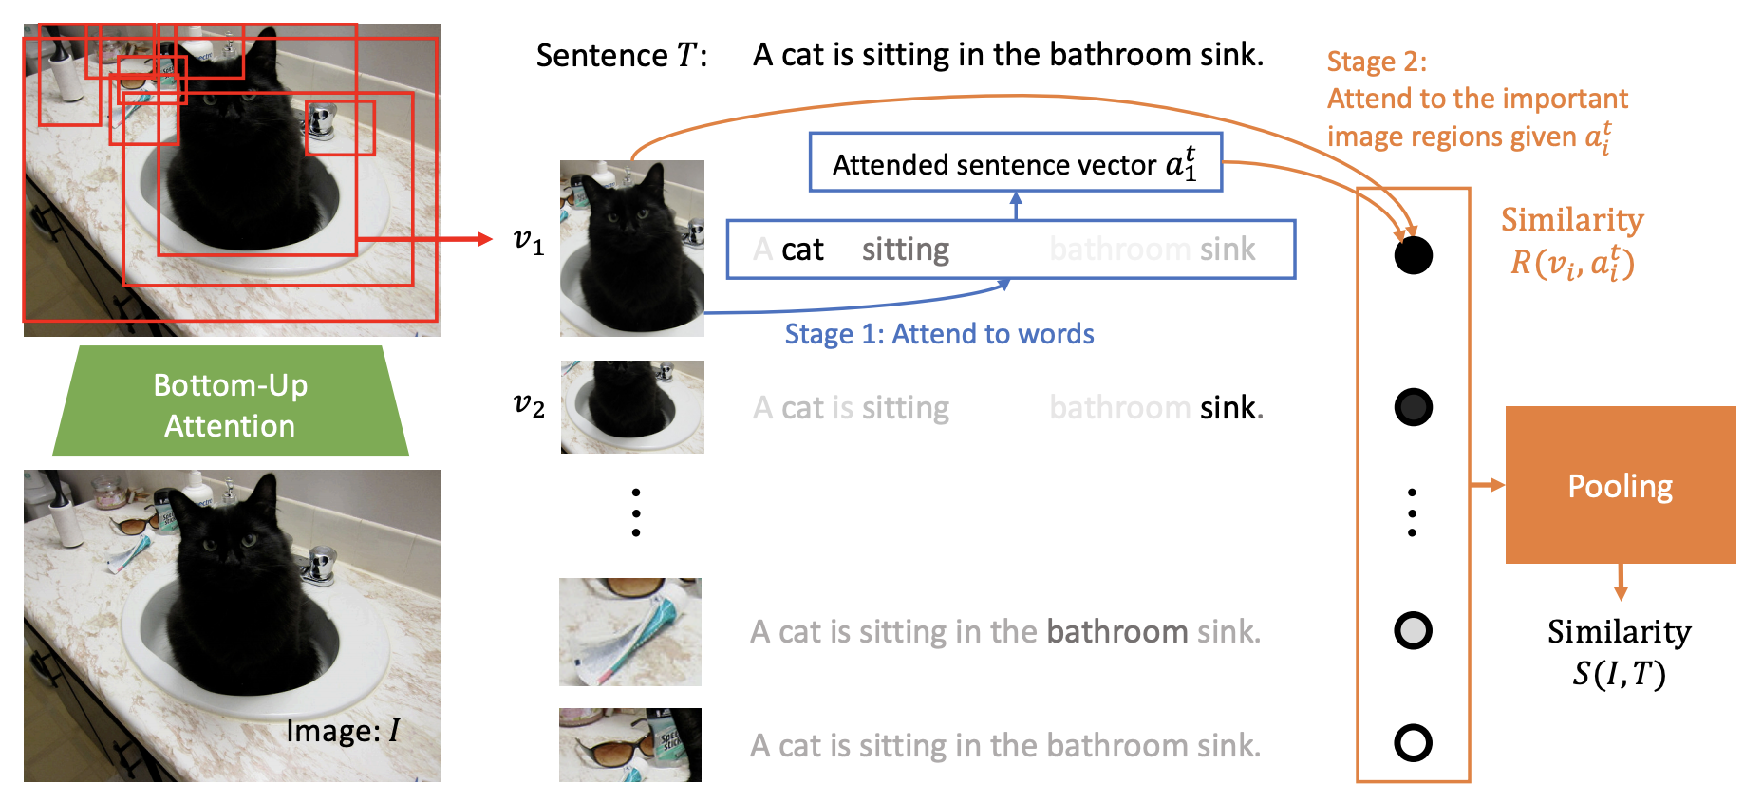
\includegraphics[width=\textwidth]{scan1.pdf}
\caption{Image-Text Stacked Cross Attention}
\label{fig:scan1}
\end{figure}

First, use bottom-up attention \cite{bottomup} to extract multiple proposals into features for the image, then map to the same dimensions as the sentence features, and use bi-direction GRU to extract features for the sentence.

Stage 1: calculate the attention representation $a_{i}^{t}$ of all words for each region $i$, and add them together to obtain the sentence representation $a_{i}^{t}$, the formula is as follows:

$$
a_{i}^{t}=\sum_{j=1}^{n} \alpha_{i j} e_{j}
$$

where

$$
\alpha_{i j}=\frac{\exp \left(\lambda_{1} \bar{s}_{i j}\right)}{\sum_{j=1}^{n} \exp \left(\lambda_{1} \bar{s}_{i j}\right)}
$$

Stage 2: calculate the cosine similarity of the $i$-th region and the obtained $a_{i}^{t}$.

$$
R\left(v_{i}, a_{i}^{t}\right)=\frac{v_{i}^{T} a_{i}^{t}}{\left\|v_{i}\right\|\left\|a_{i}^{t}\right\|}
$$

Finally, $i$ areas are superimposed together to get the similarity between image and text, using LogSumExp pooling (LSE), i.e.

$$
S_{L S E}(I, T)=\log \left(\sum_{i=1}^{k} \exp \left(\lambda_{2} R\left(v_{i}, a_{i}^{t}\right)\right)\right)^{\left(1 / \lambda_{2}\right)}
$$

Alternatively, we can
summarise $R\left(v_{i}, a_{i}^{t}\right)$ with average pooling (AVG), i.e.

$$
S_{A V G}(I, T)=\frac{\sum_{i=1}^{k} R\left(v_{i}, a_{i}^{t}\right)}{k}
$$

\subsection{Text-Image Matching}

\begin{figure}[h!]
\centering
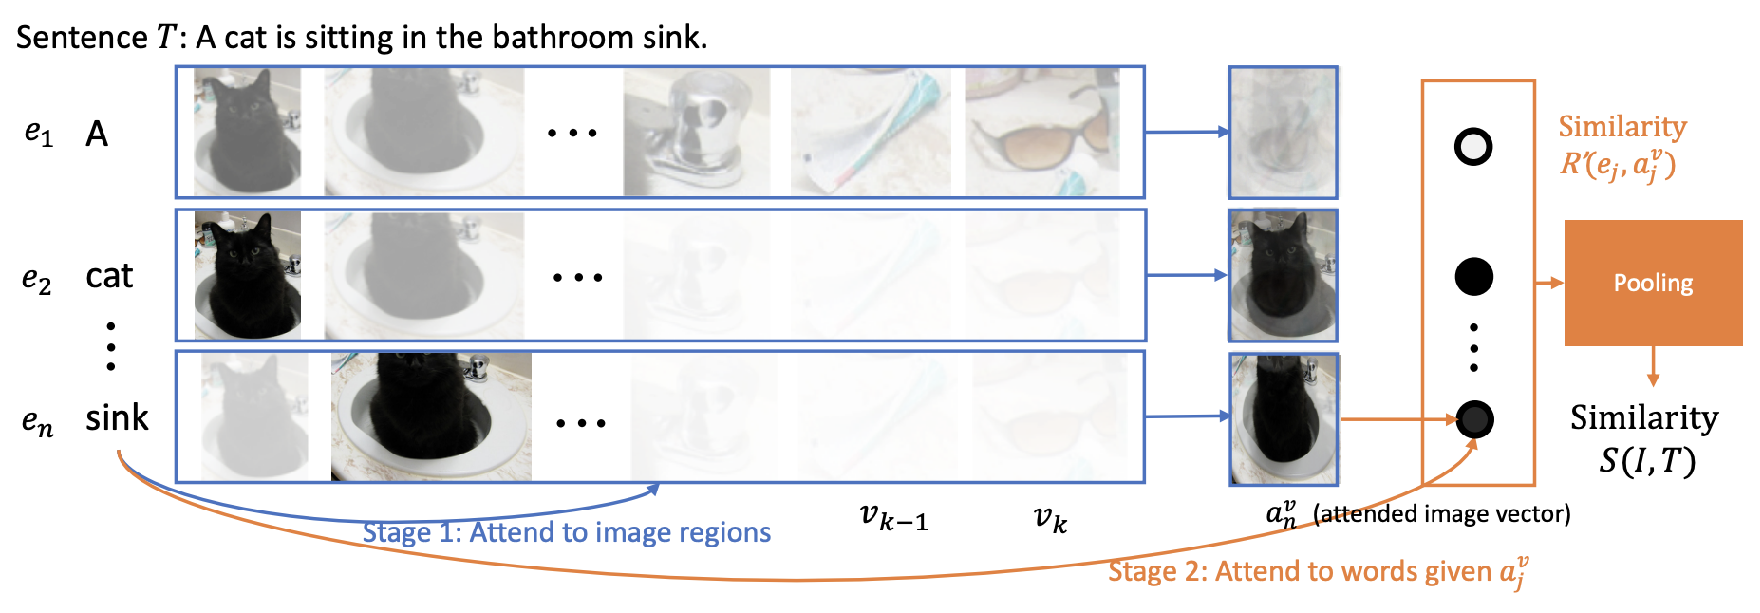
\includegraphics[width=1\textwidth]{scan2.pdf}
\caption{Text-Image Stacked Cross Attention}
\label{fig:scan2}
\end{figure}

The overall steps correspond exactly to the above, except that each word is used to calculate the similarity with the attention of a picture, which is not repeated here. The process is illustrated in Figure \ref{fig:scan2}.

\subsection{Image and Text Feature Representation}

\subsubsection{Image}Bottom-up attention technique \cite{bottomup}, which is a method of target detection, is obtained based on faster-RCNN. Faster R-CNN first obtains the area of interest for the image, and then applies a target detector to each area of interest, so that the image features can be accurately obtained.

Here the flow for image feature representation is: faster-RCNN, Residual NN (Resnet)101 $\Rightarrow$ 2,048 dimensional features $\Rightarrow$ fully-connected layer transform to $h$-dimensional $\Rightarrow$ get image feature set.

\subsubsection{Text}A RNN (recurrent neural networks) is used. Here the flow for text feature representation is: word $\Rightarrow$ one-hot vector showing an index of the word in vocab $\Rightarrow$ embed to 300-dimensional vector $\Rightarrow$ bidirectional GRU map to $h$ dimensions word feature.

\subsection{Target Alignment}
Target alignment is essentially the setting of the loss function. In this case, SCAN employs a hinge-based triplet ranking loss with margin $\alpha$.

$$
l(I, T)=\sum_{\hat{T}}[\alpha-S(I, T)+S(I, \hat{T})]_{+}+\sum_{\hat{I}}[\alpha-S(I, T)+S(\hat{I}, T)]_{+}
$$

\begin{itemize}
    \item where $[x]_{+} \equiv \max (x, 0)$ and $S$ represents the similarity score calculation function (i.e. $S_{L S E}$)
    \item The first sum calculates all negative sentences retrieval result $\hat{T}$ given an image $I$ input and the second sum takes over all negative images retrieval result $\hat{I}$ given a sentence $T$ input.
    \item If an image $I$ and a sentence $T$ are closer to one another in the joint common space than any negative pairs, the hinge loss is zero by the margin $\alpha$,.
\end{itemize}

Here we only consider the hard negatives in a mini-batch of stochastic gradient descent instead of summing over all the negative samples to make the calculations more computational efficient.

\begin{itemize}
    \item for a pair $(I, T)$, the formula is shown below. e.g. the hard negative of one image is the image that has the highest similarity with the text besides this original pair. (vice versa for text)
    \item Now the hardest negatives are given by $$\hat{I}_{h}=\operatorname{argmax}_{m \neq I} S(m, T)$$ and $$\hat{T}_{h}=\operatorname{argmax}_{d \neq T} S(I, d)$$
    \item The final loss is: 
    $$l_{h a r d}(I, T)=\left[\alpha-S(I, T)+S\left(I, \hat{T}_{h}\right)\right]_{+}+\left[\alpha-S(I, T)+S\left(\hat{I}_{h}, T\right)\right]_{+}$$
\end{itemize}

%% SHURONG: MOVE THIS PART ABOVE THE ALIGNMENT OBJECTIVE. REPRESENT THE SENTENCE AND IMAGES WITH CORRECT mathematical symbols (these symbols should be consistent both in the representation part and alignment objective part)[done]

%% SHURONG: Replace the results and examples with full image-sentence related stuff because text here is fine-grained [done]
\section{Preliminary Results}
Here we perform SCAN on two artwork datasets introduced in Chapter \ref{cha:intro}: one ancient Egyptian artworks and one Chinese artworks. For ancient Egyptian artworks dataset, it has 14,353 images in the training set, 1,793 images in the testing/validation set. The other Chinese artworks dataset, there are 6,086 images in the training set, 761 images in the testing and validation set each.

For experiment settings, we tested on a Ubuntu machine with Intel Xeon Processor E5-1620 (10M Cache, 3.60 GHz) CPU and a GeForce GTX TITAN X GPU. The specific parameters settings are listed below:

\subsubsection{Settings for image representation}

\begin{itemize}
    \item We used faster R-CNN model and ResNet-101 model pre-trained by \textit{Anderson et al.} on \verb|Visual Genomes| dataset, performs detection of salient regions as bottom-up attention to extract features from images. 
    \item To perform retrieval on a coarse-grained level, we use whole images as input. Instead of capturing multiple ($k>1$) Region of Interests (ROIs) for each image, here we set $k=1$ which captures all full images after average pooling and extracted 2,048-dimensional features vector.
    \item We used L2 normalisation (Euclidean distance) into 1,024 joint common spaces (same for GRU), these will be used as image feature vectors.
\end{itemize}

\subsubsection{Settings for text representation}

\begin{itemize}
    \item We obtained 300 dimensional word embedding as input to GRU then use embedding matrix to map it into 1,024 joint embedding spaces.
\end{itemize}

\subsection{Evaluation Metrics}

Recall is one of the most commonly used metrics in the field of information retrieval. Here in this research project, we evaluate the performance of sentence retrieval (image query) and image retrieval (sentence query) by the recall at $K$ (R@$K$). This is defined as the fraction of queries for which the correct item is retrieved in the closest $K$ points to the query. 

\subsection{Results}

The following Table \ref{table:resultscan} illustrates the results of running SCAN model on our ancient Egyptian and Chinese art alignment datasets.

\begin{table}[h!]
\centering
\begin{tabular}{lllllll}
\hline\hline
                       & \multicolumn{3}{c}{Sentence Retrieval} & \multicolumn{3}{c}{Image Retrieval} \\ \hline
Method                 & R@1         & R@5         & R@10       & R@1        & R@5        & R@10      \\ \hline\hline
\multicolumn{1}{r}{}   & \multicolumn{6}{c}{Ancient Chinese Art Alignment Dataset}                   \\ \hline
SCAN i-t AVG & 15.3        & 38.5        & 49.9       & 14.1       & 37.6       & 50.2      \\ \hline\hline
\multicolumn{1}{r}{}   & \multicolumn{6}{c}{Ancient Egyptian Art Alignment Dataset}                    \\ \hline
SCAN i-t AVG & 3.3         & 20.4        & 36.1       & 8.0        & 22.9       & 33.8 \\\hline\hline     
\end{tabular}
\caption{Result of SCAN on Artwork Datasets}
\label{table:resultscan}
\end{table}

The results are beyond satisfactory as shown; however, as in this stage, we only used the features obtained using bottom-up attention \cite{bottomup} to train and test, the result may be misleading. As bottom-up attention model was trained on natural images, which means the features we obtained for training and testing set may be irrelevant to those contained in artworks. Noted using an entire artwork image and a sentence caption to feed SCAN may also lose detailed information in artworks, which will be further discussed in Chapter \ref{cha:Method}.

\subsection{Examples}
Below we display a few examples from our coarse-grained cross modal retrieval model: one for each dataset under sentence retrieval and image retrieval.

\subsubsection{Sentence Retrieval}
Figure \ref{fig:scani2t} illustrates two examples which obtained sentences from full image queries. There are several characteristics were successfully obtained from the left Egyptian anthropoid statue and the right Chinese vase including the shape and colour but not in a more detailed level. That is, for example, our textual retrieval results captured ``\textit{human-headed}human-headed'', ``\textit{white glassy porcelain vase}'' and even a little bit detail: ``\textit{colourful patterns on the body}'', however, more details need to be furnished such as ``\textit{long thin beard}'' and ``\textit{flowering begonia, iris, and butterfly}''. These cannot be accomplished well under the current settings we used which is coarse-grained based on image and sentence level.

\begin{figure}[h!]
\centering
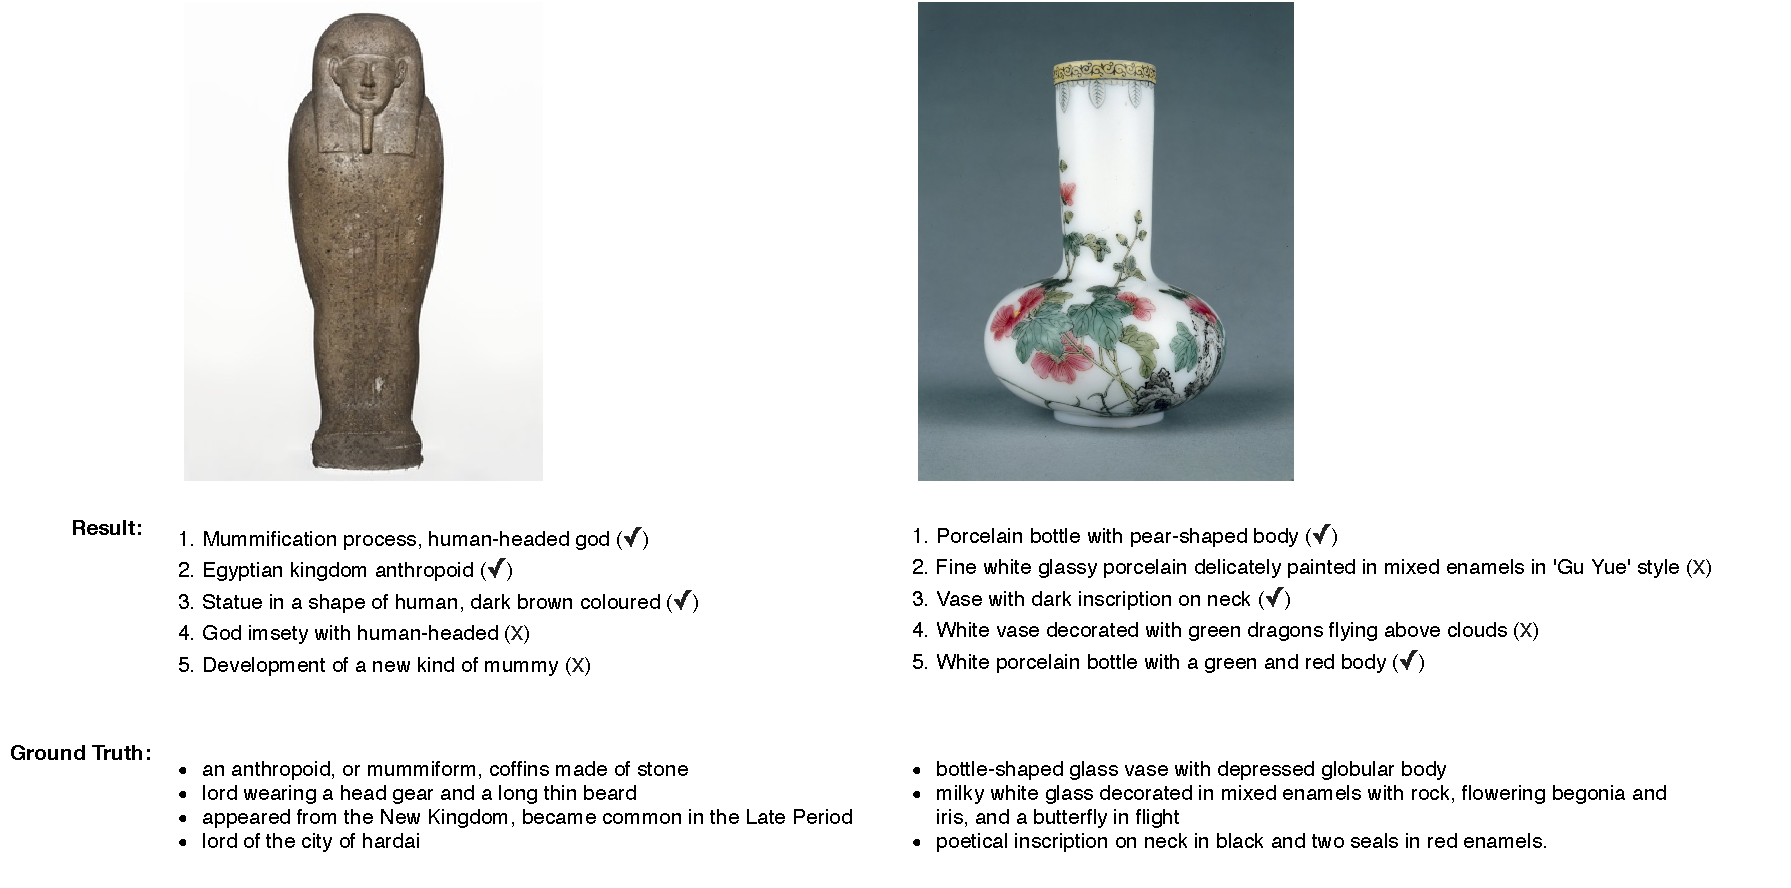
\includegraphics[width=\textwidth]{scani2t.pdf}
\caption{Sentence Retrieval Example for Given Image Queries (coarse-grained)}
\label{fig:scani2t}
\end{figure}

\subsubsection{Image Retrieval}
Similar results appeared in image retrieval examples shown as Figure \ref{fig:scant2i}. The model was able to pick out major shapes and overall structure but detailed information cannot be well aligned between full images and sentences thus cause inaccurate retrieval on a more fine-grained level.

\begin{figure}[h!]
\centering
\includegraphics[width=\textwidth]{scant2i.pdf}
\caption{Image Retrieval Example for Given Sentence Queries (coarse-grained)}
\label{fig:scant2i}
\end{figure}

There is a significant issue in under the current model: too many irrelevant textual attributes in our training data - especially our Egyptian dataset. These adjuncts, preposition and conjunctions are often noises comparing to the noun phrases, which generally contain essential information of artwork descriptions. For instance, in the process of text-image stacked cross attention, we first attend words to image fragments and then attend to words given attended image vector. These produced attended image vectors may lose some degree of accuracy when these noisy words took part in the attention steps. Therefore, some subtle, detailed features may not be correctly captured by SCAN while mixing with noises. To solve this drawback, we make some changes to SCAN in the next Section.


\section{Conclusion}
Automated image-text mutual annotation would help to transform traditional library artwork collection to digital. In this chapter, we employed a well-known cross modal retrieval model: Stacked Attention and evaluated our Egyptian and Chinese artwork datasets on it. Considering the unique representation of artworks and the rich information they usually contain, in the next chapter, we modify this current model to perform the cross modal retrieval task at a fine-grained level.


%%% Local Variables: 
%%% mode: latex
%%% TeX-master: "thesis"
%%% End: 
